\section{Aumentación de tiempo de reverberación}
El proceso de aumentación de respuestas al impulso puede realizarse tomando como parámetros del proceso cierto descriptores temporales como el tiempo de reverberación $TR_{60}$. Esto es, partiendo de una respuesta al impulso con un $TR_{60}$ determinado, se busca generar nuevas respuestas al impulso cuyo $TR_{60}$ pueda ser controlado paramétricamente para ocupar de manera homogenea y balanceada un rango de valores de interés. 
El $TR_{60}$ se relaciona directamente con la forma de la envolvente de caida de nivel exponencial presente en la parte tardia de las respuestas al impulso. El proceso de aumentación equivale a modificar esta pendiente de caida, multiplicando la señal original por una nueva envolvente que produzca el efecto deseado en la envolvente resultante. Los pasos a seguir para realizar este proceso son: 

\begin{itemize}
  \item Acondicionamiento de la respuesta al impulso de entrada.
  \item Filtrado por bandas de octava o bandas de tercio de octava.
  \item Estimación de piso de ruido.
  \item Estimación de envolvente de caida.
  \item Sintetizar una señal aplicando la envolvente estimada con piso de ruido cero a una señal de ruido Gaussiano. 
  \item Realizar el cross-fade entre la señal sintetizada y la señal original en el punto inicial del piso de ruido.
  \item Aumentación de la envolvente de caida multiplicando la señal por la correspondiente envolvente exponencial creciente/decreciente.
  \item Suma de las sub-bandas para obtener la señal resultante en su espectro completo.
  \item Integración de la parte tardia aumentada con la parte temprana de la respuesta al impulso inicial.
\end{itemize} 	

A continuación se explica cada paso del algoritmo con mayor profundidad.
%Acondicionamiento
En primer lugar, se define una determinada frecuencia de muestro y profundidad de bits para trabajar con la señal de entrada, en este caso una respuesta al impulso real. Una vez asegurada la homogeneidad de estas caracteristicas, la señal se normaliza para trabajar en un rango de amplitud acotado en el intervalo $[-1,1]$ y luego se separa la parte temprana de la parte tardia de la respuesta al impulso. Esto ultimo se realiza aplicando ventanas temporales de acuerdo a lo que indican las ecuaciones \ref{eqn:early} y \ref{eqn:late}, utilizando una ventana de tolerancia de $t_{0} = 2.5 ms$. Para los pasos siguientes se trabaja únicamente modificando la parte tardia, y la parte temprana se almacena para ser utilizada en el paso final a la hora de reconstruir la respuesta completa. En la figura \ref{fig:impulso_entrada} se  muestra la respuesta al impulso desde la que se parte, distinguiendo la descomposición temporal de la misma y luego la parte tardia de la respuesta al impulso aislada con la que se va a trabajar durante el proceso.

\begin{figure}[H]
	\centering{}
	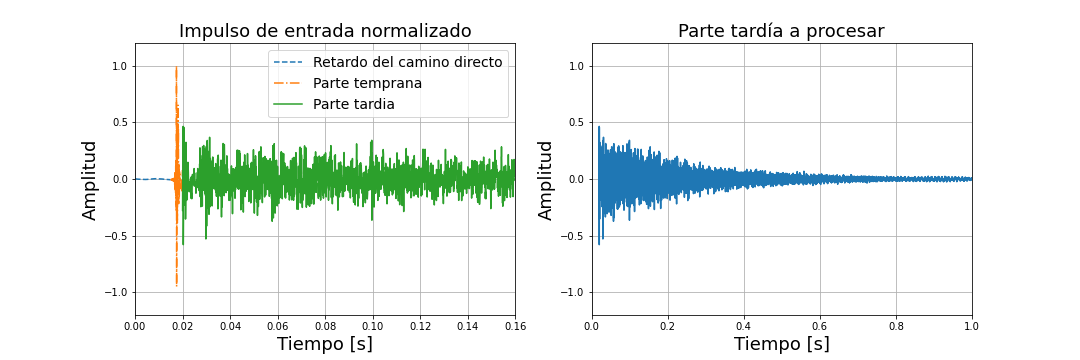
\includegraphics[scale=0.45]{impulso_entrada.png}
	\caption{Descomposición de la respuesta al impulso a procesar durante la aumentación temporal}
	\label{fig:impulso_entrada}
\end{figure}

Luego, el siguiente paso consiste en descomponer la señal en bandas de octava o tercios de octava. En esta demostración se trabaja con bandas de octava desde $125 \ Hz$ hasta $4000 \ Hz$ teniendo en cuenta que se trabaja con una fruecuencia de muestreo de $16000$ muestras por segundo. Es necesario trabajar en sub-bandas frecuenciales para contemplar la dependencia del tiempo de reverberación con la frecuencia, y mantener esa característica en las señales a generar en este proceso. Para conseguir esta descomposición en sub-bandas frecuenciales se crea un banco de filtros. El mismo se compone de filtros Butterworth que van siendo creados a partir de las frecuencias centrales que se quiera obtener en cada banda. El proceso consiste en crear filtros pasa-banda para generar una banda de paso alta y una banda de paso baja. Luego, se toma la banda de paso alta y se la vuelve a dividr en banda de paso alta y baja aplicando un nuevo par de filtros pasa-banda. Esto se repite hasta completar todas las frecuencias de corte necesarias. De esta forma se obtiene el prototipo IIR de cada filtro que compone el banco de filtros. Una vez obtenido esto, se crean respuestas de tipo FIR para cada filtro a traves de pasar un impulso ideal por cada filtro. En la figura \ref{fig:banco_filtros} se puede observar la respuesta en frecuencia del banco de filtros. Un detalle importante a considerar es que la suma del efecto de todos los filtros es unitaria para todo el rango frecuencial analizado, siendo esta una caracteristica necesaria para poder descomponer la señal en bandas y luego re-componer la señal sumando las bandas sin generar ningun tipo de distorsión en el proceso. Para lograr esto, los coeficientes de los filtros deben ser elevados al cuadrado (lo que equivale poner dos filtros en cascada) para lograr que en las intersecciones entre los filtros la suma de ampliuntud sea unitaria (en la frecuencia de corte se genera una caida de 6 dB en lugar de los 3 dB que presentaria in filtro Butterworth simple). 

\begin{figure}[H]
	\centering{}
	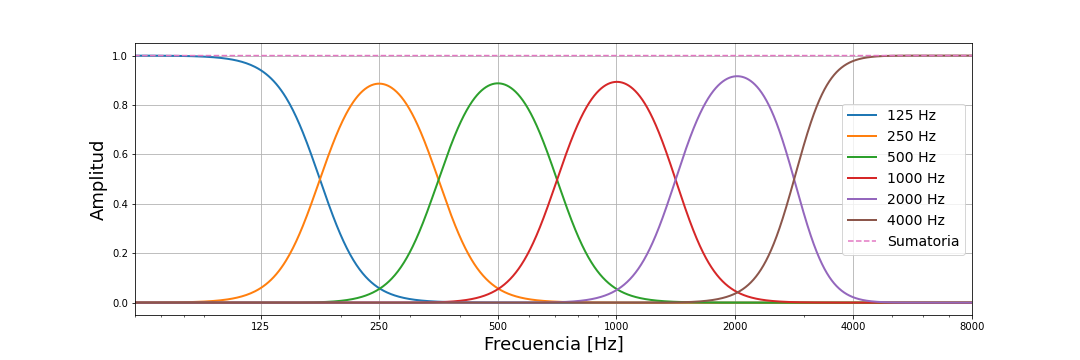
\includegraphics[scale=0.45]{banco_filtros.png}
	\caption{Banco de filtros Butterworth}
	\label{fig:banco_filtros}
\end{figure}

A partir de aplicar este banco de filtros, la señal de entrada se descompone en 6 sub-bandas como se muestra en la figura \ref{fig:sub_bandas}. En este grafico se puede apreciar como la pendiente de caida varia segun la banda de frecuencia que se observa. Todos los procesos subsiguientes se aplican de manera independiente para cada banda, y luego al final las bandas se suman para volver a tener una señal correspondiente al espectro completo original. De ahora en adelante, por una cuestion de simplicidad se muestran los gráficos pertenecientes a la banda de $1000 Hz$ de manera ilustrativa.

\begin{figure}[H]
	\centering{}
	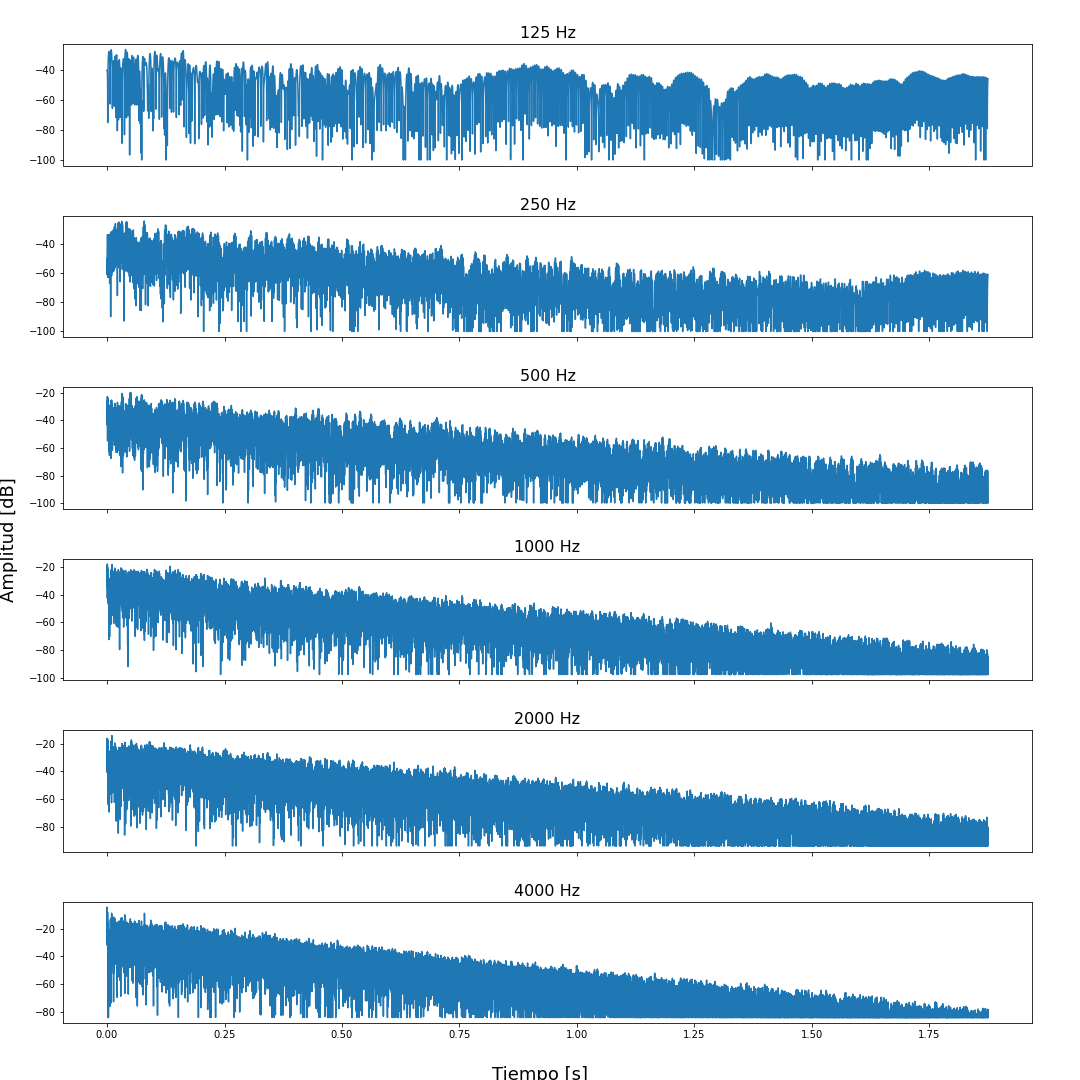
\includegraphics[scale=0.45]{sub_bandas.png}
	\caption{Sub-bandas obtenidas luego de aplicar el banco de filtros}
	\label{fig:sub_bandas}
\end{figure}

El paso siguiente consiste en determinar el piso de ruido de la señal. Detectar el piso de ruido permite asegurar que el metodo de aumentación no amplifique ruido cuando se busca obtener un tiempo de reverberación mayor al inicial propio de la respuesta al impulso de entrada. Para determinar el punto donde predomina el ruido en la respuesta al impulso se utiliza el metodo iterativo de Lundeby \cite{Lundeby}. El mismo consta de los siguientes pasos: 

\begin{enumerate}
\item La respuesta al impulso al cuadrado es promediada en intervalos de tiempo locales de entre $10 \ ms$ y $50 \ ms$ para obtener una curva 'suavizada', es decir, disminuir las variaciones instantaneas sin perder las pendientes cortas.
\item Se hace una primera estimacion del piso de ruido. Para hacerlo se toma el segmento correspondiente al ultimo $10\%$ de la respuesta al impulso.
\item La pendiente de caida se estima aplicando una regresión lineal sobre el intervalo de tiempo que contiene la respuesta entre el pico de $0 \ dB$ y el primer intervalo $5-10 \ dB$ por encima del ruido de fondo.
\item Se determina un punto de cruce provisorio en la intersección entre la pendiente de caida estimada y el nivel de piso de ruido.
\item Se obtiene un nuevo intervalo de tiempo de acuerdo a la pendiente calculada, de manera que haya entre $3$ y $10$ intervalos por cada $10 \ dB$ de caida
\item Se vuelve a promediar localmente el impulso al cuadrado de acuerdo al nuevo intervalo temporal calculado previamente 
\item Se estima el ruido de fondo nuevamente. El segmento a evaluar debe corresponder a $5-10 \ dB$ luego del punto de cruce (siguiendo la curva estimada previamente), o bien, un minimo del $10\%$ de la señal total (en el caso de tener que optar por el $10\%$ de nuevo, el resultado seria el mismo que antes, y el punto encontrado previamente seria el definitivo).
\item Se estima la pendiente de caida para un rango dinamico de entre $20 \ dB$ y $10 \ dB$, empezando desde un punto $5-10 \ dB$ por encima del nivel de ruido.
\item Se encuentra un nuevo punto de cruce.
\item Los pasos 7-9 se repiten hasta que el valor del piso de ruido converja, tolerando un maximo de 6 iteraciones.
\end{enumerate}

El paso siguiente es estimar la pendiente paramétrica que mejor se aproxime a la pendiente de caida real. La estimación se basa en el modelo de la ecuación \ref{eqn:decay_exp}. Por lo tanto, los parámetros que se busca estimar son la amplitud inicial, la tasa de caida y el nivel de piso de ruido. La estimación se realiza aplicando un algoritmo de ajuste no lineal por cuadrados mínimos. El resultado de la estimación para la banda de $1000 Hz$ se muestra en la figura  \ref{fig:estimacion_parametrica}.

\begin{figure}[H]
	\centering{}
	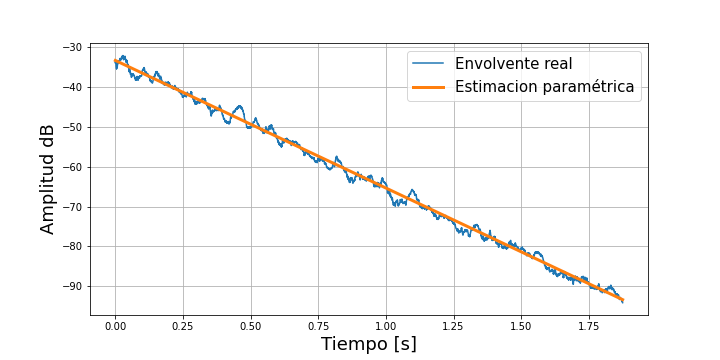
\includegraphics[scale=0.45]{estimacion.png}
	\caption{Estimación paramétrica de la pendiente de caida.}
	\label{fig:estimacion_parametrica}
\end{figure}

Con estos parámetros estimados se genera una nueva envolvente de caida pero llevando el nivel de piso de ruido a cero, y se aplica esta envolvente sobre una señal de ruido Gaussiano de media cero y desvio estandar unitario. Con esta señal sintética y la señal original se hace una trasición cruzada en el punto estimado del piso de ruido. De esta manera se elimina el ruido de la señal original, reemplazadolo por la caida exponencial determinada por la envolvente paramétrica.  En la figura \ref{fig:recorte_ruido} se puede observar como se extiende la respuesta luego del punto de inicio del piso de ruido de la señal original.

\begin{figure}[H]
	\centering{}
	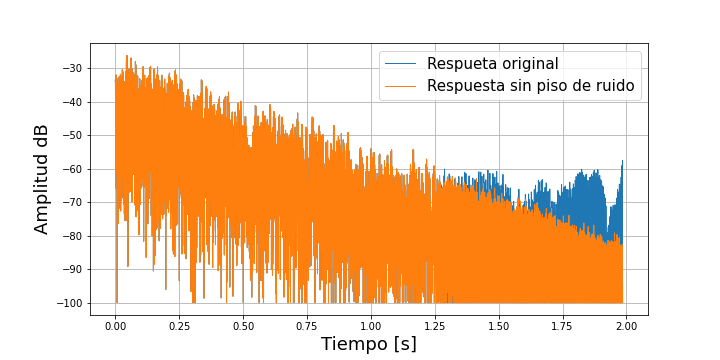
\includegraphics[scale=0.45]{recorte_ruido.png}
	\caption{Respuesta original y extendida sin piso de ruido.}
	\label{fig:recorte_ruido}
\end{figure}

Finalmente, teniendo las bandas extendidas habiendose eliminado el piso de ruido, se prosigue con el proceso de aumentación del tiempo de reverberación para cada sub-banda, multiplicando cada respuesta por la correspondiente envolvente exponencial creciente o decreciente segun corresponda, para obtener la envolvente de caida necesaria para generar el tiempo de reverberación deseado, como se indica en la ecuación \ref{eqn:aug_tr}. Un ejemplo del resultado de la aumentación sobre una sub-banda de frecuencia se muestra en la figura \ref{fig:banda_aumentada}, en donde el tiempo de reverberación objetivo es menor que el tiempo de reverberación de la respuesta original, por lo cual la pendiente aumentada resulta mas atenuada que la pendiente original. 

\begin{figure}[H]
	\centering{}
	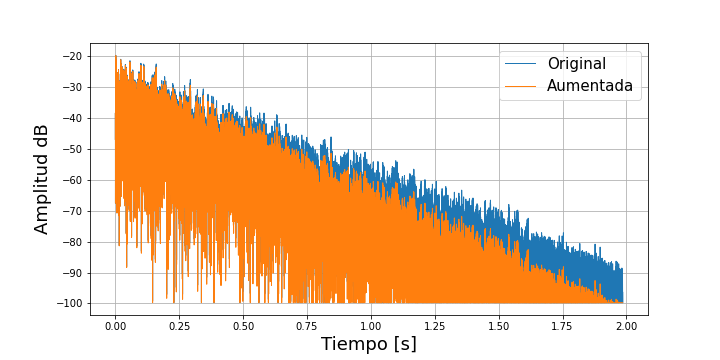
\includegraphics[scale=0.45]{banda_aumentada.png}
	\caption{Aumentación del tiempo de reverberación alterando la envolvente de caida original.}
	\label{fig:banda_aumentada}
\end{figure}

Una vez realizada la alteración de la envolvente de caida para todas las bandas frecuenciales, estas se suman para conformar nuevamente la parte tardia de la respuesta al impulso de espectro completo. El paso final consiste en concatenar los segmentos de la respuesta al impulso original que no fueron alterados, es decir, el delay del camino directo y la parte temprana de la respuesta. Con esto, el proceso de aumentación termina, y se obtiene como resultado una nueva respuesta al impulso con el tiempo de reverberación deseado. En la figura \ref{fig:salida_aumentacion_tr} se muestra la respuesta al impulso original comparada con la nueva respuesta generada a partir del proceso anteriormente descripto. 

\begin{figure}[H]
	\centering{}
	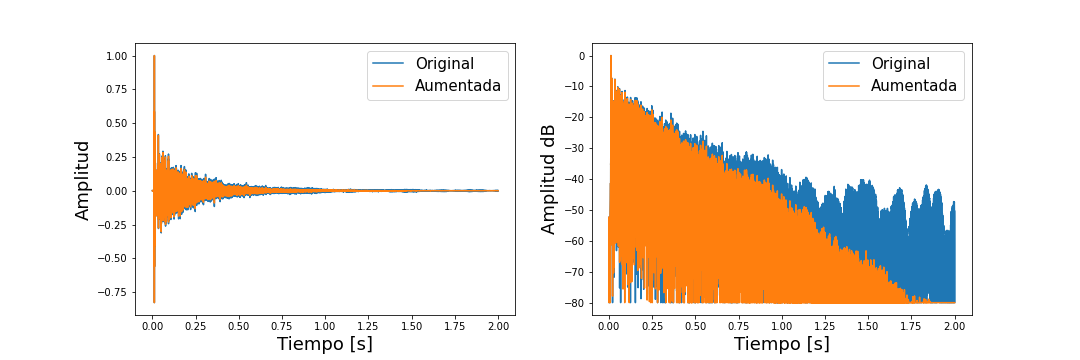
\includegraphics[scale=0.45]{tr_aug.png}
	\caption{Resultado del proceso de aumentación del tiempo de reverberación de una respuesta al impulso}
	\label{fig:salida_aumentacion_tr}
\end{figure}






